\documentclass[10pt]{article}
\usepackage[utf8]{inputenc}
\usepackage{amsmath}
\usepackage{amsfonts}
\usepackage{amssymb}
\usepackage{amsthm}
\usepackage{graphicx}
\usepackage{enumerate}
\usepackage{ragged2e}
\usepackage[spanish,onelanguage]{algorithm2e}
%\setlength{\parindent}{0em}
\usepackage[left=3cm,right=3cm,top=2cm,bottom=2.5cm]{geometry}
\usepackage{tikz}
\usepackage{tikz-cd}
\author{Ángel Ríos San Nicolás}
\theoremstyle{definition}
\newtheorem{ejer}{Ejercicio}
\newtheorem*{sol}{Solución}
\title{Geometría Discreta y Computación}
\date{Hoja 1--Politopos cíclicos, matroides orientadas.\\11 de enero de 2020}

\begin{document}
\maketitle
\begin{ejer}Recuérdese que el politopo cíclico $C(d,n)$ se define como la envolvente convexa de $n$ puntos tomados en orden a lo largo de la curva de momentos $c(t)=(t,\ldots,t^d)$.
\begin{enumerate}[(a)]
\item Dado un subconjunto $S$ de $[n]=\{1,\ldots,n\}$ con $|S|=d$, $[n]\setminus S$ es un cocircuito (por ser la matroide uniforme), y que el correspondiente \textit{cocircuito orientado} consiste en partir $[n]\setminus S$ en dos trozos de acuerdo con el signo del funcional afín que se hace cero en el hiperplano $\text{aff}(S)$. Extender el criterio de paridad de Gale a la siguiente caracterización de los cocircuitos orientados de $C(d,n)$: dos elementos $a,b\notin S$ están en el mismo lado del cocircuito si, y solo si $[a,b]\cap S$ es par.
\item Demostrar que los circuitos orientados de $C(d,n)$ son todos los subconjuntos de tamaño $d+2$ de $[n]$, partidos en dos de manera alternada. Es decir, los pares de la forma $$\left(\left\{i_1,i_3,\ldots\right\},\left\{i_2,i_4,\ldots\right\}\right)$$
donde $i_1<i_2<\cdots<i_{d+2}.$
\end{enumerate}

\end{ejer}
\begin{sol}\leavevmode
\begin{enumerate}[(a)]
\item Sea $S\subseteq [n]$ tal que $|S|=d$ y existe un funcional afín $f:\mathbb{R}^d\longrightarrow\mathbb{R}$ con $f(S)=0$. El funcional está dado por $f(x_1,\ldots, x_d)=\alpha_1x_1+\cdots + \alpha_d x_d$ con $\alpha_1,\ldots,\alpha_d\in\mathbb{R}$. Restringiendo a la curva de momentos, tenemos la función polinomial $\tilde{f}(t)=f(c(t))=\alpha_1t+\cdots+\alpha_d t^d$ que se anula en el  conjunto $S=\{s_1,\ldots, s_d\}$, por tanto, $\tilde{f}(t)=\alpha_d(t-s_1)\cdots (t-s_d)$, donde podemos suponer sin pérdida de generalidad que $\alpha_d>0$ tomando el funcional opuesto si es necesario. Sean $a,b\notin S$. Queremos controlar el signo del funcional en $a$ y $b$ que indica a qué parte del cocircuito pertenece cada uno. De la descomposición anterior tenemos que
\begin{align*}
     &\text{sign}\left(\tilde{f}(a)\right) =  \prod_{i=1}^d\text{sign}(a-s_i) = (-1)^{|(-\infty,b]\cap S|}\\
    & \text{sign}\left(\tilde{f}(b)\right) =  \prod\limits_{i=1}^d\text{sign}(b-s_i)  =  (-1)^{|[a,\infty)\cap S|}
\end{align*}
Multiplicando, deducimos cuándo $a$ y $b$ están en la misma parte del cocircuito orientado.
$$\text{sign}\left(\tilde{f}(a)\right)\text{sign}\left(\tilde{f}(b)\right)=(-1)^{|(-\infty,b]\cap S|+|[a,\infty)\cap S|}=(-1)^{|[a,b]\cap S|}$$
Por definición, $a$ y $b$ están en la misma parte del cocircuito si y solo si el funcional tiene el mismo signo en $a$ y en $b$, es decir, cuando el producto anterior
es positivo o, equivalentemente, cuando $|[a,b]\cap S|$ es par como queríamos probar.

% Si $a$ y $b$ están al mismo lado del cocircuito, suponemos sin pérdida de generalidad que están en el lado positivo, es decir, $f(c(a))>0$ y $f(c(b))>0$. Supongamos que $[a,b]\cap S$ es impar. Por el criterio de paridad de Gale, $S$ no define una faceta del politopo cíclico.

% Si $[a,b]\cap S$ es par, razonamos por reducción al absurdo. Suponemos que están en distinto lado del cocircuito, es decir, sin pérdida de generalidad $f(c(a))<0$ y $f(c(b))>0$. Debe existir $i_0\in S$ tal que $s_{i_0}\in [a,b]\cap S$.

\item Por ser la matroide de las independencias afines del politopo cíclico de dimensión $d$, es una matroide uniforme de rango $d+1$ con lo que todo conjunto con $d+2$ elementos es dependiente minimal, es decir, un circuito.
Dado un circuito $X=\{i_1,i_2,\ldots, i_{d+2}\}\subseteq [n]$. Para todos $k,l\in\{1,\ldots, d+2\}$ con $k<l$, consideramos $S_{k,l}=X\setminus\{i_k,i_l\}$ que es un subconjunto de $[n]$ con $d$ elementos. Sabemos que determina un cocircuito $C_{k,l}=[n]\setminus S_{k,l}$. Claramente, el circuito $X$ y el cocircuito $C_{k,l}$ tienen exactamente dos elementos en común, $i_k$ e $i_l$. Si en uno tienen signos distintos, en el otro tienen el mismo, pero el signo en el cocircuito está determinado por la paridad de $|[i_k,i_l]\cap S_{k,l}|$ salvo tomar la orientación opuesta. Se cumple que $|[i_k,i_l]\cap S_{k,l}|$ es par si y solo si $k-l$ es par porque solo contamos los elementos en $S$. Por tanto, $i_k$ e $i_l$ están en distintas componentes del circuito si y solo si $k$ y $l$ tienen distinta paridad.
\end{enumerate}
\end{sol}
\begin{ejer}Calcular el chirotopo, los circuitos orientados, y los cocircuitos orientados, de las siguientes configuraciones de vectores de rango tres:
\begin{enumerate}[(a)]
    \item La configuración ``no Fano", dada por las columnas de la siguiente matriz:
    $$F:=\overset{\begin{matrix}1 & 2 & 3 & 4 & 5 & 6 & 7\end{matrix}}{\overline{\begin{pmatrix}1 & 0 & 0 & 0 & 1 & 1 & 1 \\
    0 & 1 & 0 & 1 & 0 & 1 & 1\\
    0 & 0 & 1 & 1 & 1 & 0 & 1\end{pmatrix}}}$$
    \item Las ``raíces positivas del sistema de Coxeter de tipo $A_3$", dadas por las columnas de la siguiente matriz:
    $$A_3^+:=\overset{\begin{matrix}1 & 2 & 3 & 4 & 5 & 6\end{matrix}}{\overline{\begin{pmatrix}1 & 0 & 0 & 0 & 1 & 1 \\
    0 & 1 & 0 & 1 & 1 & 1\\
    0 & 0 & 1 & 1 & 0 & 1\end{pmatrix}}}$$
\end{enumerate}
Demostrar que el segundo es una matroide gráfica, pero el primero no.

\end{ejer}

\begin{sol}\leavevmode
\begin{enumerate}[(a)]
\item El chirotopo de la matroide dada por $F$ es la aplicación $$\chi : E^3\longrightarrow \{-1,0,1\}, (v_1,v_2,v_3)\longmapsto \chi(v_1,v_2,v_3)=\text{sign}(|v_1,v_2, v_3|)$$
que aplica cada $3$-tupla de $E$ en el signo de su determinante siendo $E$ el conjunto de vectores columna de $F$. Como abuso de notación, consideramos $E=\{1,\ldots, 7\}$. Tenemos que calcular el signo de todos los posibles determinantes $3\times 3$. Por la antisimetría del determinante (o del chirotopo), podemos calcular los determinantes salvo permutaciones. Las permutaciones pares conservan el signo y las impares lo cambian. Los determinantes con columnas repetidas son claramente nulos. No detallamos los cálculos, se puede calcular fácilmente desarrollando por filas o columnas.

$$\begin{array}{l|l|l|l|l}
\chi(123)=1 & \chi(234)=0 & \chi(345)=-1 & \chi(456)=1 & \chi(567)=1\\
\chi(124)=1 & \chi(235)=1 & \chi(346)=-1 & \chi(457)=1 &\\
\chi(125)=1 & \chi(236)=1 & \chi(347)=-1 & \chi(467)=-1& \\
\chi(126)=0 & \chi(237)=1 & \chi(356)=1 & & \\
\chi(127)=1 & \chi(245)=1 &\chi(357)=1 & &\\
\chi(134)=-1 & \chi(246)=1 &\chi(367)=0 & &\\
\chi(135)=0 & \chi(247)=1& & &\\
\chi(136)=-1 & \chi(256)=1 & & &\\
\chi(137)=-1 & \chi(257)=0 & & &\\
\chi(145)=1 &\chi(267)=-1 & & &\\ 
\chi(146)=-1 & & & &\\
\chi(147)=0 & & & &\\
\chi(156)=-1 & & & &\\
\chi(157)=-1 & & & &\\
\chi(167)=1 & & & &\\
\end{array}$$

Los circuitos orientados son los conjuntos dependientes minimales dotados de orientación. Los conjuntos dependientes minimales se corresponden a conjuntos con una única dependencia lineal y la orientación a la elección de los signos. Por construcción, la matriz no tiene columnas de ceros ni múltiplos de otras con lo que los circuitos tienen al menos tres vectores.

Para calcular los circuitos con tres vectores, fijamos dos vectores y buscamos, si lo hay, otro vector linealmente dependiente. Los circuitos orientados de tamaño tres son:
$$\begin{array}{cc|cc}
     (\{1,2\},\{6\})& (\{6\},\{1,2\}) & (\{2,3\},\{4\}) & (\{4\},\{2,3\})\\
     (\{1,3\},\{5\})& (\{5\},\{1,3\}) & (\{2,5\},\{7\}) & (\{7\},\{2,5\})\\
     (\{1,4\},\{7\}) & (\{7\},\{1,4\}) & (\{3,6\},\{7\}) & (\{7\},\{3,6\})\\
\end{array}$$

Por ejemplo, las posibles orientaciones del primer circuito $(\{1,2\},\{6\})$, $(\{6\},\{1,2\})$ se tienen de las igualdades 
$$\begin{array}{ll}\begin{pmatrix}1\\ 0\\ 0\end{pmatrix} + \begin{pmatrix}0\\ 1\\ 0\end{pmatrix}-\begin{pmatrix}1\\ 1\\ 0\end{pmatrix}=0 & -\begin{pmatrix}1\\ 0\\ 0\end{pmatrix}-\begin{pmatrix}0\\ 1\\ 0\end{pmatrix}+\begin{pmatrix}1\\ 1\\ 0\end{pmatrix}=0\end{array}$$
y están determinadas por los signos de los coeficientes. Análogamente para el resto de circuitos orientados.


Para calcular los circuitos de cuatro vectores, fijamos tres columnas linealmente independientes (información que obtenemos del chirotopo). Para cada columna distinta, o bien el conjunto contiene un circuito de tamaño tres previamente calculado (no minimalidad), o bien genera una única combinación lineal con el resto, es decir, que quitando cualquier columna se tiene un conjunto linealmente independiente (minimalidad). Los circuitos orientados son la información de los signos de la combinación lineal. Los circuitos orientados de tamaño cuatro son:
$$\begin{array}{cc}
(\{1,2,3\},\{7\}) & (\{7\},\{1,2,3\})\\
(\{1,4\},\{2,5\}) & (\{2,5\},\{1,4\})\\
(\{1,4\},\{3,6\}) & (\{3,6\},\{1,4\})\\
(\{1,4\},\{5,6\}) & (\{5,6\},\{1,4\})\\
(\{1,7\},\{5,6\}) & (\{5,6\},\{1,7\})\\
(\{2,5\},\{3,6\}) & (\{3,6\},\{2,5\})\\
(\{2,5\},\{4,6\}) & (\{4,6\},\{2,5\})\\
(\{2,7\},\{4,6\}) & (\{4,6\},\{2,7\})\\
(\{2,7\},\{4,6\}) & (\{4,6\},\{2,7\})\\
(\{3,7\},\{4,5\}) & (\{4,5\},\{3,7\})\\
(\{4,5,6\},\{7\}) & (\{7\},\{4,5,6\})\\
\end{array}$$


No hay circuitos de tamaño mayor que $4$ porque el rango de la matriz es $3$. Cualquier tal conjunto de vectores es linealmente dependiente aun quitando un vector, con lo que no es un circuito por no ser minimal.

Para calcular los cocircuitos orientados, fijamos dos columnas linealmente independientes de la matriz y buscamos un funcional lineal que se anule en ellas. El cocircuito orientado es el vector de signos del funcional en las columnas en que no se anula. Para cada funcional lineal podemos considerar el opuesto y obtenemos así dos cocircuitos orientados. Denotamos los funcionales lineales $f:\mathbb{R}^3\longrightarrow\mathbb{R}$ por su imagen sobre $(x_1,x_2,x_3)\in\mathbb{R}$. Los cocircuitos orientados son:

$$\begin{array}{|c|c|c|c|c|}
\hline f & f^{-1}(0) & E\setminus f^{-1}(0) & \multicolumn{2}{c|}{\text{Cocircuitos orientados}} \\
\hline x_1 & \{2,3,4\} & \{1,5,6,7\} & (\{1,5,6,7\},\emptyset) & (\emptyset,\{1,5,6,7\})\\
\hline x_2 & \{1,3,5\} & \{2,4,6,7\} &  (\{2,4,6,7\},\emptyset) & (\emptyset,\{2,4,6,7\})\\
\hline x_3 & \{1,2,6\} & \{3,4,5,7\} & (\{3,4,5,7\},\emptyset) & (\emptyset,\{3,4,5,7\})\\
\hline x_1-x_2 & \{3,6,7\} & \{1,2,4,5\} & (\{1,5\},\{2,4\}) & (\{2,4\},\{1,5\})\\
\hline x_1-x_3 & \{2,5,7\} & \{1,3,4,6\} & (\{1,6\},\{3,4\}) & (\{3,4\},\{1,6\})\\
\hline x_2-x_3 & \{1,4,7\} & \{2,3,5,6\} &  (\{2,6\},\{3,5\}) & (\{3,5\},\{2,6\})\\
\hline x_1+x_2-x_3 & \{4,5\} & \{1,2,3,6,7\} & (\{1,2,6,7\},\{3\}) & (\{3\},\{1,2,6,7\})\\
\hline x_1-x_2-x_3 & \{5,6\} & \{1,2,3,4,7\} & (\{1\},\{2,3,4,7\}) & (\{2,3,4,7\},\{1\})\\
\hline x_1-x_2+x_3 & \{4,6\} & \{1,2,3,5,7\} & (\{1,3,5,7\},\{2\}) & (\{2\},\{1,3,5,7\})\\
\hline
\end{array}$$
% Podemos representar geométricamente la matroide dada por $F$ como
% \begin{center}
% \begin{tikzpicture}
% \draw [thick] (-1,-1) -- (1,-1);
% \draw [thick] (1,-1) -- (0,1);
% \draw [thick] (0,1) -- (-1,-1);
% \draw [thick] (0.5,0) -- (0,0);
% \draw [thick] (-0.5,0) -- (0,0);
% \draw [thick] (0,1) -- (0,0);
% \draw [thick] (0,0) -- (0,-1);
% \filldraw (-1,-1) circle (2.5pt) node[left] {2};
% \filldraw (1,-1) circle (2.5pt) node[right] {3};
% \filldraw (0,1) circle (2.5pt) node[above] {1};
% \filldraw (0,0) circle (2.5pt) node[anchor=south east] {7};
% \filldraw (0.5,0) circle (2.5pt) node[right] {5};
% \filldraw (-0.5,0) circle (2.5pt) node[left] {6};
% \filldraw (0,-1) circle (2.5pt) node[below] {4};
% \end{tikzpicture}
% \end{center}
\item El chirotopo de la matroide orientada dada por $A_3^+$ es una restricción del chirotopo de la matroide dada por $F$. La matriz es la misma que la anterior salvo que no tenemos la columna $\begin{pmatrix}1 & 0 & 1\end{pmatrix}^t$.
Como antes, calculamos el chirotopo salvo permutaciones y columnas repetidas:
$$\begin{array}{l|l|l|l}
\chi(123)=1 & \chi(234)=0 & \chi(345)=-1 & \chi(456)=-1\\
\chi(124)=1 & \chi(235)=1 & \chi(346)=-1 &\\
\chi(125)=0 & \chi(236)=1 & \chi(356)=0 &\\
\chi(126)=1 & \chi(245)=1 & &\\
\chi(134)=-1 & \chi(246)=1 & &\\
\chi(135)=-1 & \chi(256)=-1 & &\\
\chi(136)=-1 & & &\\
\chi(145)=-1 & & &\\
\chi(146)=0 & & &\\
\chi(156)=1 & & &\\
\end{array}$$

Los circuitos orientados de tamaño tres son:

$$\begin{array}{cc}
    (\{1,2\},\{5\}) & (\{5\},\{1,2\}) \\
    (\{1,4\},\{6\}) & (\{6\},\{1,4\}) \\
    (\{2,3\},\{4\}) & (\{4\},\{2,3\}) \\
    (\{3,5\},\{6\}) & (\{6\},\{3,5\}) 
\end{array}$$

Los circuitos orientados de tamaño cuatro son:
$$\begin{array}{cc}
    (\{1,2,3\},\{6\}) & (\{6\},\{1,2,3\}) \\
    (\{1,4\},\{3,5\}) & (\{3,5\},\{1,4\}) \\
    (\{2,6\},\{4,5\}) & (\{4,5\},\{2,6\}) \\
\end{array}$$

Los cocircuitos orientados son:

$$\begin{array}{|c|c|c|c|c|}
\hline f & f^{-1}(0) & E\setminus f^{-1}(0) & \multicolumn{2}{c|}{\text{Cocircuitos orientados}} \\
\hline x_1 & \{2,3,4\} & \{1,5,6\} & (\{1,5,6\},\emptyset) & (\emptyset,\{1,5,6\})  \\
\hline x_2 & \{1,3\} & \{2,4,5,6\} & (\{2,4,5,6\},\emptyset) & (\emptyset,\{2,4,5,6\})  \\
\hline x_3 & \{1,2,5\} & \{3,4,6\} & (\{3,4,6\},\emptyset) & (\emptyset,\{3,4,6\}) \\
\hline x_1-x_2 & \{3,5,6\} & \{1,2,4\} & (\{1\},\{2,4\}) & (\{2,4\},\{1\})  \\
\hline x_1-x_3 & \{2,6\} & \{1,3,4,5\} & (\{1,5\},\{3,4\}) & (\{3,4\},\{1,5\})  \\
\hline x_2-x_3 & \{1,4,6\} & \{2,3,5\} & (\{2,5\},\{3\}) & (\{3\},\{2,5\})  \\
\hline x_1-x_2+x_3 & \{4,5\} & \{1,2,3,6\} & (\{1,3,6\},\{2\}) & (\{2\},\{1,3,6\})  \\
\hline
\end{array}$$

% Podemos representar geométricamente la matroide dada por $A_3^+$ como
% \begin{center}
% \begin{tikzpicture}
% \draw [thick] (-1,-1) -- (1,-1);
% \draw [thick] (0,1) -- (-1,-1);
% \draw [thick] (0,1) -- (0,0);
% \draw [thick] (0,0) -- (0,-1);
% \filldraw (-1,-1) circle (2.5pt) node[left] {2};
% \filldraw (1,-1) circle (2.5pt) node[right] {3};
% \filldraw (0,1) circle (2.5pt) node[above] {1};
% \filldraw (0,0) circle (2.5pt) node[anchor=south east] {6};
% \filldraw (-0.5,0) circle (2.5pt) node[left] {5};
% \filldraw (0,-1) circle (2.5pt) node[below] {4};
% \end{tikzpicture}
% \end{center}

\end{enumerate}
Un grafo de la matroide de las raíces positivas del sistema de Coxeter de tipo $A_3$ es 
\begin{center}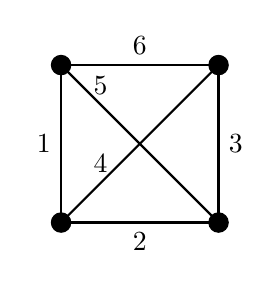
\begin{tikzpicture}
\draw [thick] (-1,-1) -- (1,-1) node[midway,sloped,below] {2};
\draw [thick] (-1,-1) -- (-1,1) node[midway,left] {1};
\draw [thick] (-1,1) -- (1,1) node[midway,above] {6};
\draw [thick] (1,-1) -- (1,1) node[midway,right] {3};
\draw [thick] (-1,-1) -- (1,1) node[midway,near start,above]{4};
\draw [thick] (-1,1) -- (1,-1) node[midway,near start,above]{5};
\filldraw (1,1) circle (3.5pt);
\filldraw (-1,-1) circle (3.5pt);
\filldraw (1,-1) circle (3.5pt);
\filldraw (-1,1) circle (3.5pt);
\end{tikzpicture}\end{center}
Observamos que la información de qué aristas del grafo forman ciclos es precisamente la matroide que queríamos.

Para probar que la matroide dada por la configuración ``no Fano" no es gráfica, razonamos por reducción al absurdo. Si la matroide ``no Fano" es gráfica, entonces es la matroide de un grafo que podemos suponer conexo, sin lazos ni aristas múltiples porque no hay columnas repetidas ni múltiplos. El grafo contiene como subgrafo un grafo de la matroide anterior porque solo se diferencian en una arista, la dada por la quinta columna de $F$. Pero todo grafo de la matroide anterior cumple que las aristas $1$ y $3$ no inciden en un mismo vértice. Añadiendo una única arista $e$, podemos crear un lazo o, como mucho, conectar las componentes conexas en un árbol, pero nunca crear un ciclo formado por las aristas $1, 3$ y $e$. Esto es una contradicción con el hecho de que la arista $e$ forme un ciclo en el grafo de la matroide. Por lo tanto, la matroide ``no Fano" no es gráfica.
\end{sol}
\end{document}
